%% LyX 1.6.4 created this file.  For more info, see http://www.lyx.org/.
%% Do not edit unless you really know what you are doing.
\documentclass[oneside,bahasa,english]{scrbook}
\usepackage[T1]{fontenc}
\usepackage[latin9]{inputenc}
\setcounter{secnumdepth}{3}
\setcounter{tocdepth}{3}
\usepackage{float}
\usepackage{graphicx}

\makeatletter
%%%%%%%%%%%%%%%%%%%%%%%%%%%%%% Textclass specific LaTeX commands.
\newenvironment{lyxcode}
{\par\begin{list}{}{
\setlength{\rightmargin}{\leftmargin}
\setlength{\listparindent}{0pt}% needed for AMS classes
\raggedright
\setlength{\itemsep}{0pt}
\setlength{\parsep}{0pt}
\normalfont\ttfamily}%
 \item[]}
{\end{list}}

\makeatother

\usepackage{babel}

\begin{document}

\chapter{Modul Absensi (Penghitungan Pengunjung)}

Modul ini dapat dipanggil melalui:
\begin{lyxcode}
http://localhost/senayan3-stable14/?p=visitor
\end{lyxcode}
Tampilan modul ini adalah sebagai berikut:

\selectlanguage{bahasa}%
\begin{center}
%
\begin{figure}[H]
\begin{centering}
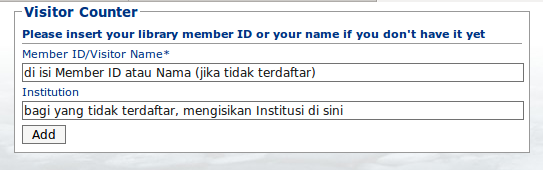
\includegraphics[scale=0.8]{image/absen-1}
\par\end{centering}

\caption{Tampilan Visitor Counter}

\end{figure}

\par\end{center}

\selectlanguage{english}%
Pengunjung perpustakaan dibedakan menjadi 2; Anggota yang sudah terdaftar
dan pengunjung yang bukan anggota/tidak terdaftar.

Jika sudah terdaftar, maka pengunjung cukup menuliskan Member ID pada
kolom atas, kemudian tekan Enter atau klik Add. Maka data sudah tersimpan
1 x kunjungan lengkap dengan jam dan tanggal kunjung. Namun jika bukan
anggota terdaftar, maka harus secara manual menuliskan Nama dan Institusi
(wajib).

Untuk keamanan dan validitas proses absensi pengunjung, Visitor Counter
ini dapat di seting hanya komputer dengan Internet Protokol tertentu
saja yang dapat mengakses. Pengaturan ini terdapat dalam file visitor.inc.php
yang ada dalam folder /senayan/lib/contents/visitor.inc.php. Scriptnya
adalah sebagai berikit:

\$allowed\_counter\_ip = array('127.0.0.1');

Pada script diatas, 127.0.0.1 merupakan IP address yang diijinkan
untuk mengakses visitor counter. Jika ada lebih dari satu komputer
maka IP Address komputer yang bersangkutan harus diisikan didalam
script diatas. Misalnya, komputer dengan IP 10.45.1.1, 10.45.1.2 dan
10.45.1.3, maka penulisannya adalah:

\$allowed\_counter\_ip = array('10.45.1.1, 10.45.1.2,10.45.1.3');

Laporan kunjungan ini dapat dilihat pada modul reporting.
\end{document}
